\chapter{Making Equipment}
Equipment creation is handled outside of specific characters. Objects created are available to all characters. For copyright reasons, there is no equipment database included, so you will have to fill it yourself.  To do so, select 'Start Equipment Database' from the Extras menu.

\paragraph{Note:} Freshly added objects will only show up in characters that are opened after the object was created. To see the object in an open character, close the character and reload it.

\section{Equipment Concepts}
<<<<<<< .mine
Everything a character can own is represented by an "object". Objects have a name, description and are made of one or more of the magical materials. Note that objects are independent of rulesets - a daiklave is a daiklave, no matter whether you play under Exalted Power Combat or Second Edition rules.

Rules are distinguished for the object's various statistics, or "stats" for short. An object can have any number of stats for any and all of the supported rulesets.

\section{Equipment Screen Breakdown}
\begin{figure}
	\centering
		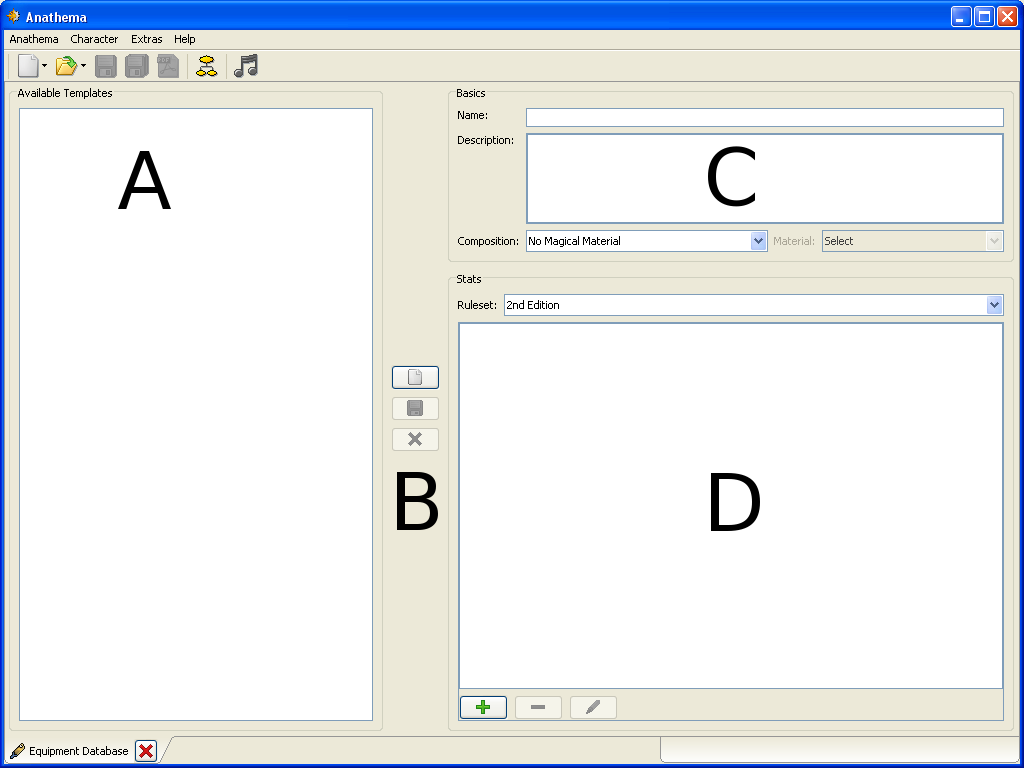
\includegraphics[width=1.00\textwidth]{images/Equipment.png}
	\caption{Equipment Database Screen}
	\label{fig:Equipment}
\end{figure}

The equipment database screen, shown in figure \ref{fig:Equipment}, consists of three parts and a set of buttons. To the left of the panel, there is a vertical list (A), showing all the objects in the database. In the center of the screen (B), buttons offer the means for general control - creating, saving and deleting objects. The right side is filled with the working area, where objects can be edited one at a time.

The working area is composed of two parts, "Basics"(C), where the object's overall details are handled, and "Stats"(D), where statistics can be added to the object. The ruleset selection box functions as both a filter for and a setting, showing only the stats for the ruleset selected and adding newly entered stats to that same ruleset. Do not be alarmed when the data you just entered disappears when you change rules, changing it back will make your hard work reappear.

To create a new object, you need to explicitly instruct the program to do so by clicking the "Create object" button (top button, showing a blank page). To edit an existing object, select it from the list to the left. 

Though the database is designed to check for changes and warn you if some or all could be lost due to your actions, you should save your progress regularly.

\section{Simple Objects}
The most simple objects consist of a name and optional description. (Don't worry about the composition and material boxes now, they will described in the "Artifacts" section below.) Once both are entered, you can save your item via the "save" button in the middle of the screen.

\paragraph{Character sheet:} These objects are neither weapons nor armor, When equipped on a character, they will be printed in the Possessions area on the second page of the character sheet.

\section{Basic Objects - Handling stats}
Basic objects venture a step further by sporting some kind of combat stats. 

To add stats, create your item as before, but instead of saving it and be done, look at the "stats" section next. 
There, you first will have to select the ruleset you want to add stats for from the combobox. Now you are ready to add stats to the object. 

Select the green + button from the stat controls at the bottom of the page to open the stat creation dialog. There, choose the type of statistics you want to add to your item. The next screens will allow you enter the various stats of the object.  You can also change the name for the set of statistics, which should only be necessary if you plan on adding multiple stats. Pressing 'Finish' will add the stats to the list in the working area.

You can remove existing stats via the '-' icon, and edit them using the pencil button on the right of the row. Thus, you can make changes without starting over.

\paragraph{Character sheet:}  A stat-set's name will only be displayed on the character sheet if you change it or if the item has multiple stat-sets.

\section{Complex Objects - Multiple stats}
You can create more complex objects by creating the base object as normal, then adding additional sets of stats.   

This method allows you to create multi-use objects like the Fighting Gauntlet, which can be used to Punch or Clinch by adding two sets of Close Combat stats (called "Punch" and "Clinch", to prevent confusion).

There is no limit to the complexity of objects created this way. You should well be able to even create warstriders with various weapons and armour statistics. 

\section{Artifacts}
Once you get beyond making mundane weapons and armor, you enter the complex realm of artifacts. Artifacts differ from mundane objects in their material composition, fittingly indicated by the "composition" box.

The 3 artifact choices offered are 'Single Material, Fixed', 'Single Material, Variable', and 'Compound'.  

\subsection{Single Material, Variable}
This is the basic option for run-of-the-mill artifacts like those listed in the core book. Choosing it tells the program that this is not a unique object but a class of artifacts. Thus, it will assume that the object receives the defaut boni granted by the magical material, and will automatically add them once the object is equipped.

Going through the steps described previously, you can select the specific object's material just before adding it to your character. The program defaults to your characters preferred material.
  
\subsection{Single Material, Fixed}
This option is used to make artifacts that are only available in one Magical Material (selected from the "Material" box to the lower right of the "basics" section).

The program assumes that there are special boni involved, and you will need to add the boni (if any) for the magical material when entering the stats for the object. Just selecting the Magical Material will not add the appropriate bonus' to the object.

\subsection{Compound}
Compound objects are made from more then one Magical Material. Generally, they do neither grant bonus the same way objects made from only one material do, nor are they restricted to only one type of exalt.  

Special boni and powers offered by these objects will have to be noted in the object's description or calculated into their statistics.